\chapter{Background}

\begin{displayquote}
``Amateur radio is a popular technical hobby and volunteer public service that uses designated radio frequencies for non-commercial exchange of messages, wireless experimentation, self-training, and emergency communications.
Amateur Radio is the only hobby governed by international treaty.'' \cite{def_amateur_radio}
\end{displayquote}

Amateur radio operators do not always sit in front of their radios. Often for operators it is more convenient to control their radios remotely, known more commonly as having a ``remote shack''. In this scenario as much remote control as possible is desired. This is often achieved using existing commercial or home made solutions that rely on simply repeating control signals. For example the ``RRC 1258Mk'' is a product designed to do just. However it is priced at \$708\cite{RRC_1258Mk} making it often prohibitively expensive as it is two times the price of budget consumer radios. Instead it would be preferable to understand and/or emulate these signals. The end result is that the radio gains \gls{cat}\cite{CAT} features.

Remote shacks are geographically positioned for their prime transceiving properties, for example on the top of a hill so the signal is less affected by the geometry of the surrounding area. They are often limited in their connectivity to utilities, such as power or Internet connection. This is especially in extremely remote areas where communication is sometimes done over telephone networks. This adds some constraints to the project and is discussed in the next section.

An ideal scenario for these kind of users is where all functions can be controlled from the radio remotely, using as little data traffic as possible. This use-case also extends to users that prefer to use a PC to control their radios. This may be for more features, better user experience (given by software), or possibly for accessibility reasons (i.e where reading the screen or using the small dials would be a problem for the operator).

\begin{figure}
    \centering
    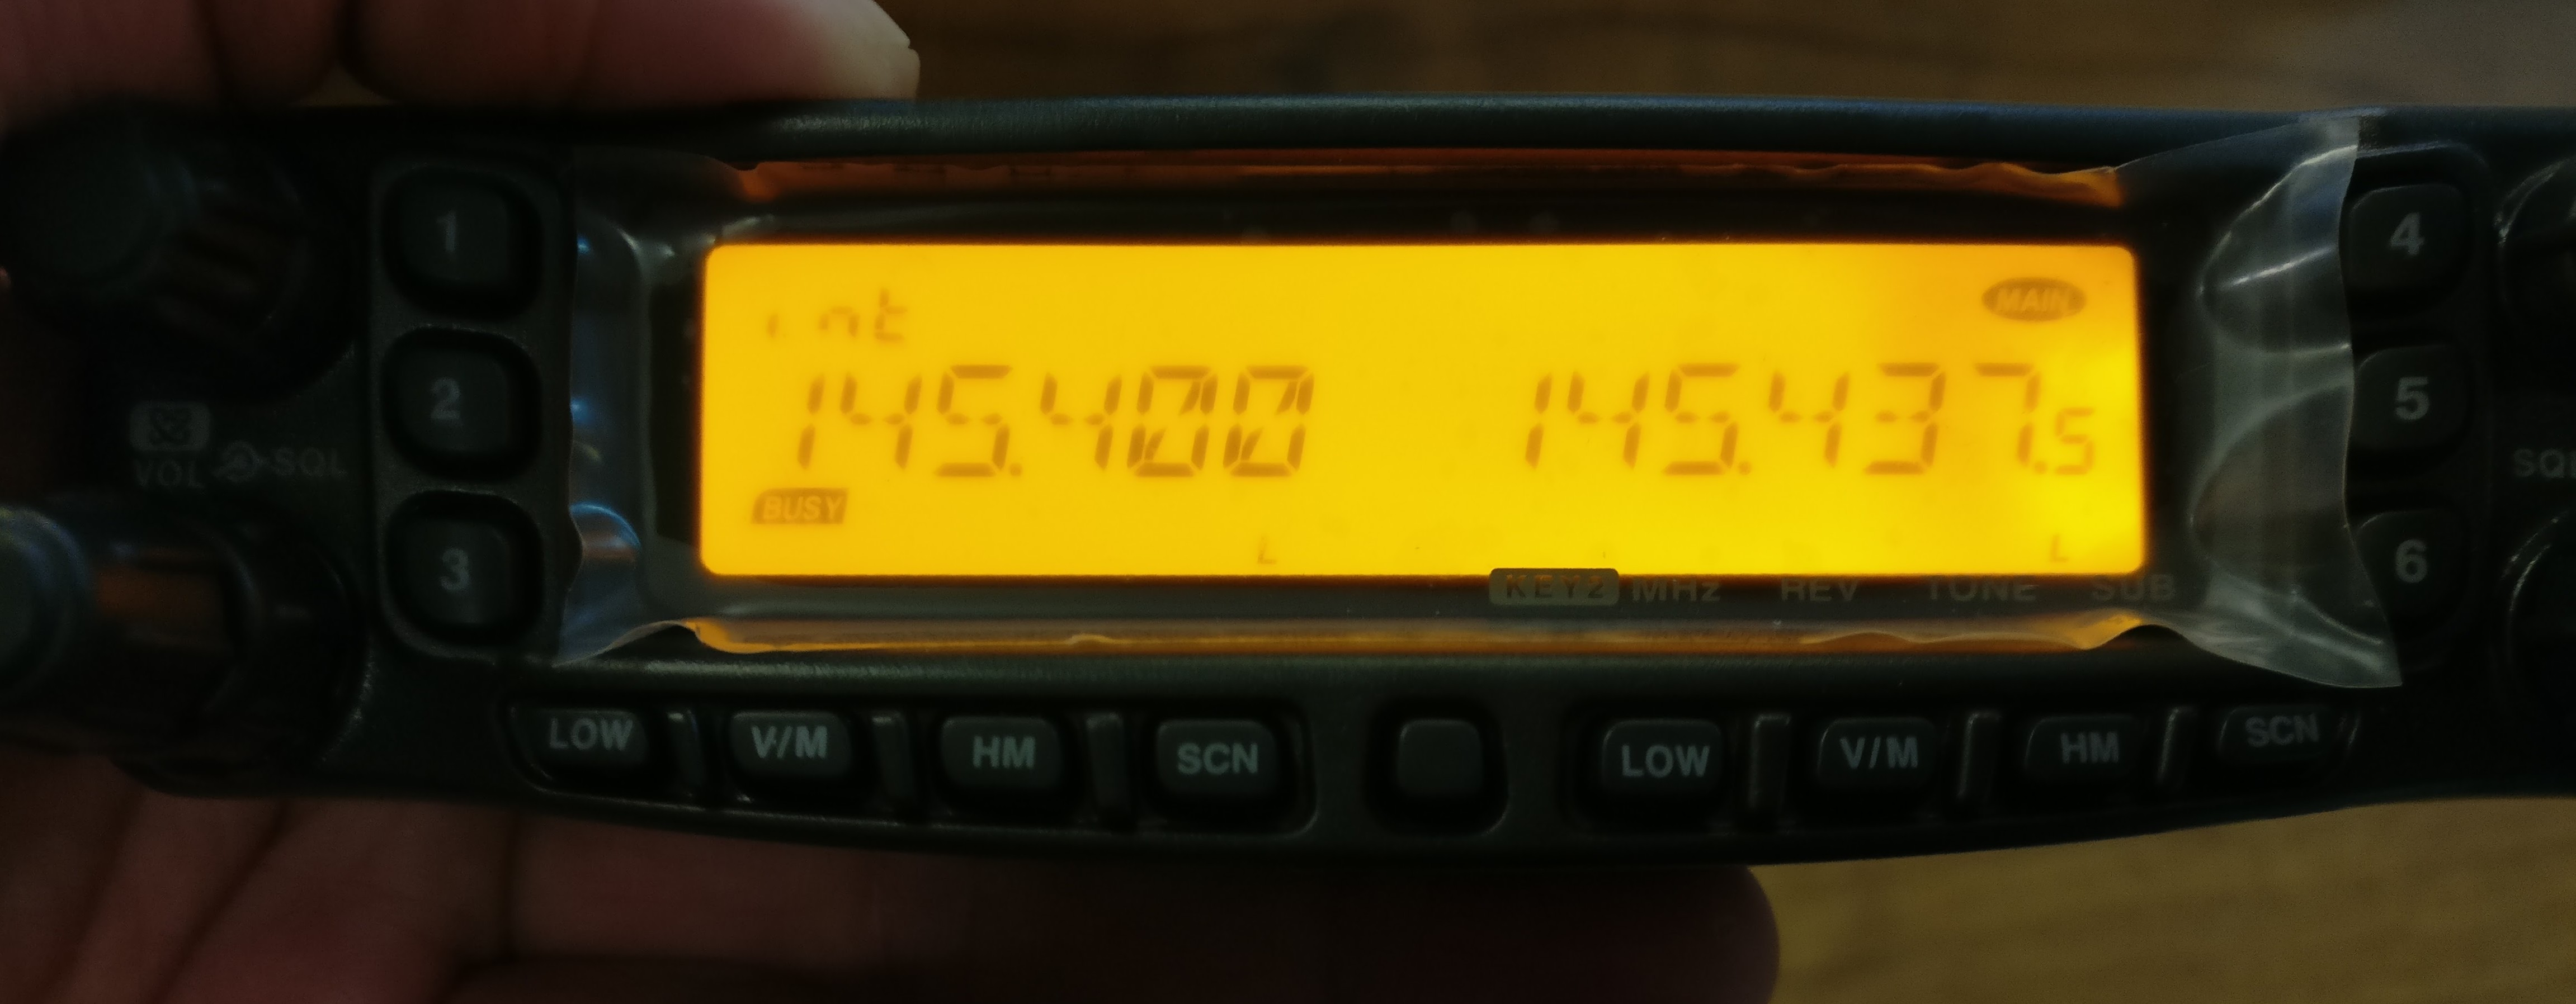
\includegraphics[width=1\textwidth]{img/radio_head}
    \caption[Picture of RT-8900r radio]{A picture of the face of the RT-8900r radio.}
    \label{fig:radio_head}
\end{figure}

The \gls{8900} (Seen in figure~\ref{fig:radio_head}) is a popular, budget amateur radio, it is marketed for mobile applications such as being mounted on a car dashboard. This is achieved using a control surface (hereby referred to as the head) that is detachable from the rest of the body of the radio. This allows the body to be mounted in a more practical location by running a control cable between the two. The \gls{8900} is capable of monitoring two separate frequencies at the same time, therefore there are duplicate controls on ether side of the radio to manipulate each receiver. The microphone connects into head and contains additional buttons such as a keypad that is able to dial a exact frequency. Conversely the loudspeaker is located in the body of the radio so a second cable must be run from the line out jack at the back of the radio to the head in order to hear audio clearly.

The main goal of this project is to allow the functions of the radio to be available from a computer. This will be achieved by adapting the \gls{8900} to have \gls{cat} features. Radios that come with this feature typically have a serial port or some kind. My project relies on the assumption that it is possible that the control line can be intercepted and emulated by a computer. This means that functionality could be added in a similar way to radios that advertise the C.A.T feature. This must be achieved cost effectively and in a simple way for the user to create and setup by themselves. Any designs and software will then be released under the GNU Public Licence (v3) for the benefit of the community.